%!TEX root = ../../main.tex


\begin{figure}[!htbp]
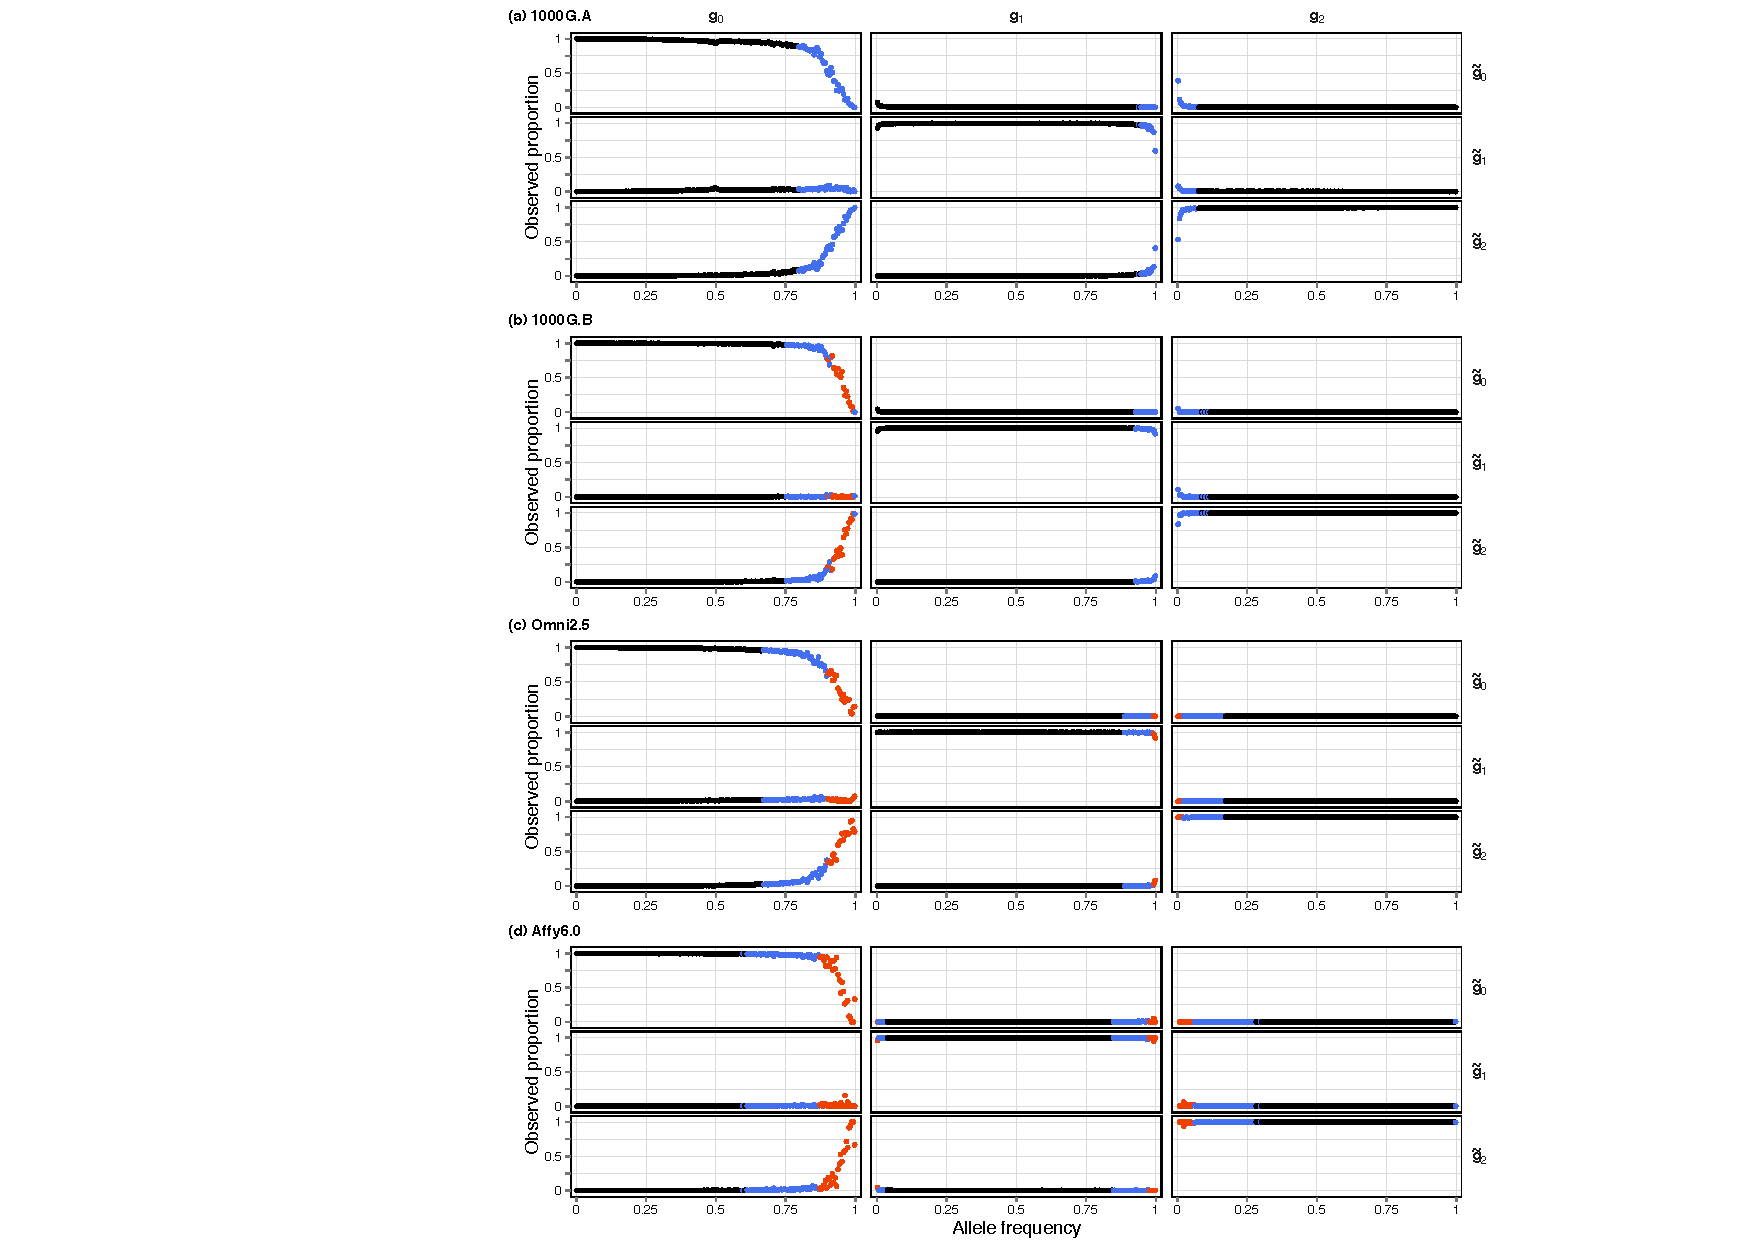
\includegraphics[width=\textwidth]{./img/ch4/generrprop}
\Caption{Frequency-dependent distribution of genotype penetrance in sequencing and genotyping data}%
{For each true genotype class (columns), the fraction of $g_j$ observed as $\tilde{g}_i$ (rows) was calculated per allele frequency bin, to estimate the frequency-dependent distribution of genotype penetrance $\varepsilon_{ij}$.
The set of matched genotypes per true genotype class was divided into \n{200} bins along the allele frequency spectrum.
Allele frequency was assigned to each matched site in a given test dataset, taking the population frequency as recorded in the full sample of the \glsentrylong{1kg} phase 3 dataset (\n{2504} individuals).
Colours indicate the number of genotypes per bin, $n$, distinguished at nominal thresholds ${N_j < 100}$ (\emph{red}), ${100 \leq N_j < 1000}$ (\emph{blue}), and ${N_j \geq 1000}$ (\emph{black}).
Note that true genotypes homozygous for the reference allele, $g_0$, were not present in \gls{ipg} and assumed from high-confidence regions if present in a given test dataset.}%
{fig:generrprop}
\end{figure}
